First, we provide a pre-processing step with the objective of having a segmented point set of the object \ref{sec:pre}. This is then used to create the probabilistic shape representation \ref{sec:object}. This is then exploited in 

%%%%%%%%%%%%%%%%%%%%%%%%%%%%%%%%%%%%%%%%
\subsection{Object Segmentation}
\label{sec:segmentation}

\citep[Sec.~III.A]{Hudson2012Endtoend} provides good candidates for object segmentation that are well oriented to object grasp, manipulation, and for our purposes, exploration. In fact, the combination of their ``Table Plane Estimation'' with their ``Volume-Based Segmentation'' yields the ubiquituos tabletop object segmentation \citep{TabletopObjectDetector}. However, to improve the rechability of the exploration, we prefer to hold the object in one hand-arm system and explore with another, as described in Sec.~\ref{sec:scope}. Thus, our selected approach for object segmentation is simpler than those approaches. The difficulties is in measuring the configuration of a soft and adaptable gripper that keeps the object in position to filter out the points belonging to the hand-arm system. For this purpose, one can rely in body-type measurements instead of traditional encoders, as described by~\citet{Santaera2015Lowcost}. Once the hand-arm system pose is measured, then a trivial passthrough filter with slightly scaled bounding boxes of the robot geometry is used to obtain a point cloud of the object isolated from the scene. Algorithm~\ref{alg:in-hand-segmentation} shows the pseudo-code of this procedure, indicating the actual. Additionally, 

It is worth noting, that this module is here just to show how visual and tactile data might be merged into a single shape model. But as a matter of fact, the initial training point set can be empty and start by simply probing naively towards the gripper to initialize the training set.

\begin{figure}
\centering
  \mbox{
  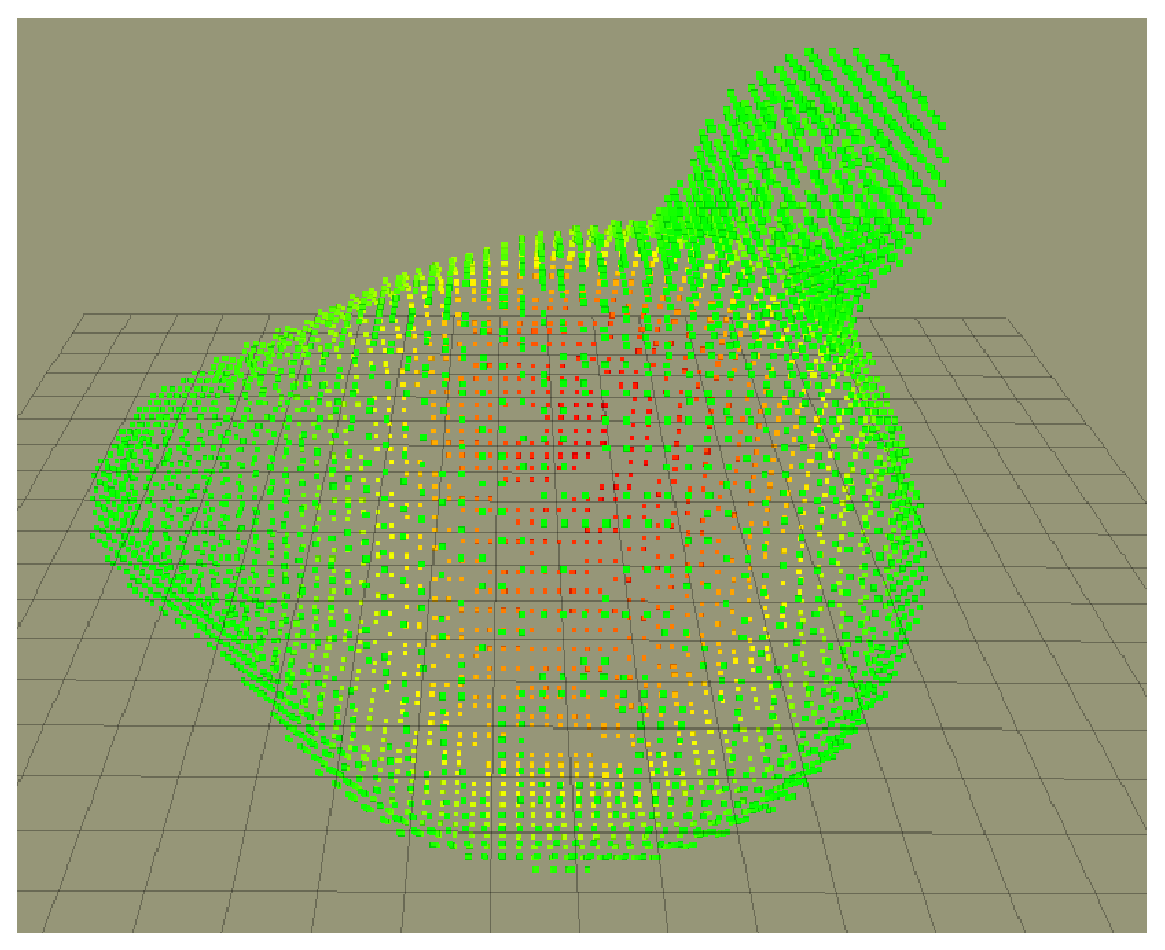
\includegraphics[width=0.45\linewidth]{example.eps}
  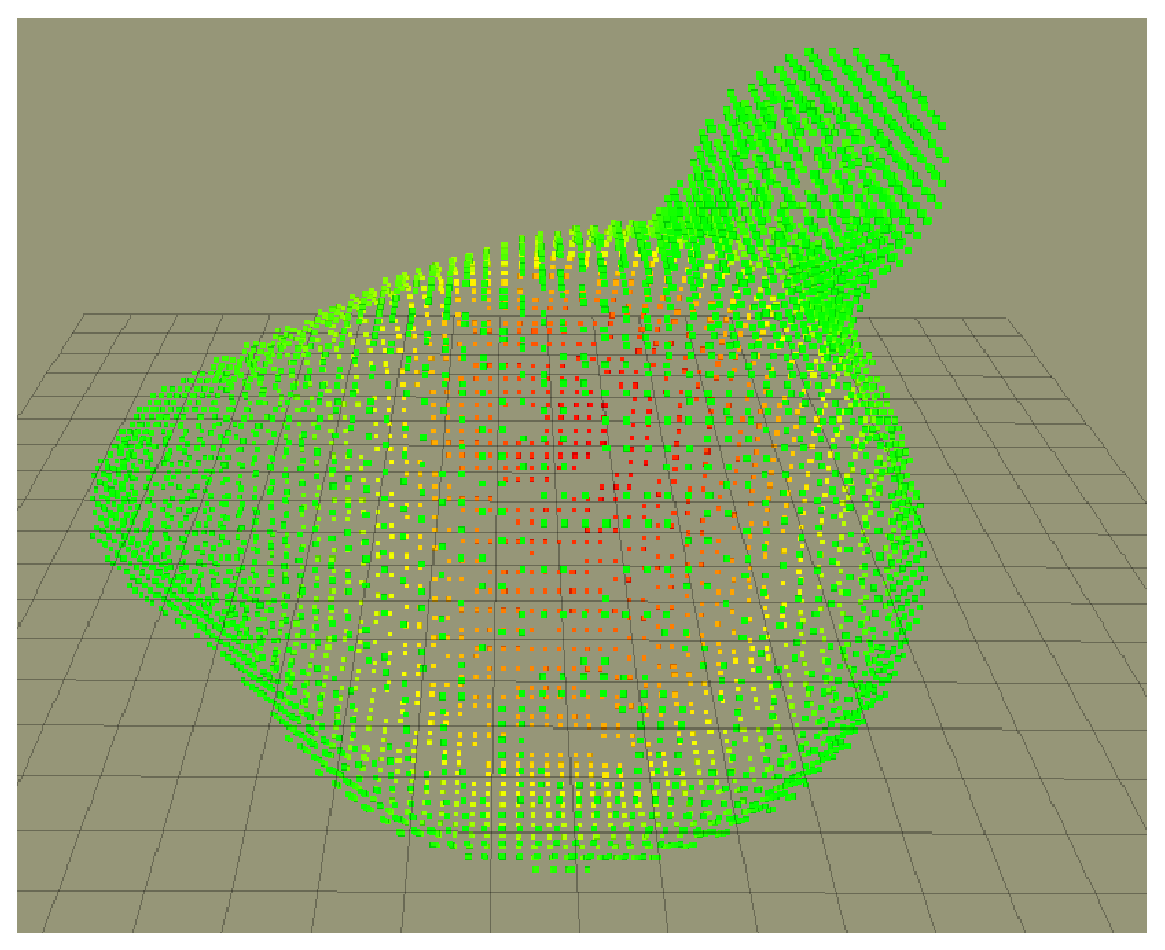
\includegraphics[width=0.45\linewidth]{example.eps}
  }
  \caption{A picture of the in-hand object segmentation using a soft-adaptive hand on a 7-dof arm in the real scene (left) and the resulting point cloud (right).} \label{fig:in-hand-segmentation}
\end{figure}

\begin{algorithm}[h]
\textbf{\textsc{segmenInHand}}$(\mathcal{R}, \kappa, \delta)$\\ %functionname
\LinesNumbered
\DontPrintSemicolon
\SetAlgoVlined \SetKwInOut{Input}{input} \SetKwInOut{Output}{output}
\Input{The point cloud of the scene $\mathcal{P}$, the robot model, $\mathcal{R}$, its visual geometry inflation factor, $\kappa$, and the downsampling resolution, $\delta$.}
\Output{The point cloud of the object isolated from the scene, $\mathcal{O}$.}
  $\mathbf{s} \leftarrow$\textsc{listenToRobotState}($\mathcal{R}$) \\
  $\mathcal{B} \leftarrow$\textsc{computeBoundingBoxes}($\mathcal{R}$, $\mathbf{s}$, $\kappa$) \\
  $\mathcal{O} \leftarrow$\textsc{applyPasstroughFilter}($\mathcal{P}$, $\mathcal{B}$) \\
  $\mathcal{O} \leftarrow$\textsc{applyDownsampleFilter}($\mathcal{O}$, $\delta$) \\
  \Return{$\mathcal{O}$}
\caption{In-hand object segmentation.} \label{alg:in-hand-segmentation}
\end{algorithm}

The \textsc{listenToRobotState}($\cdot$) method considers the measurement of soft-adaptive mechanism

%%%%%%%%%%%%%%%%%%%%%%%%%%%%%%%%%%%%%%%%
\subsection{Shape modelling}
\label{sec:shape}
What makes a good surface representation?
\begin{itemize}
\item Accurate (we handle this with probability)
\item Concise (we might want this)
\item Intuitive specification (we don't need this)
\item Local support
\item Affine invariant 
\item Arbitrary topology (we need this)
\item Guaranteed continuity (we need this)
\item Natural parameterization (we don't need this)
\item Efficient display (we shouldn't need this)
\item Efficient intersections (we could need this)
\end{itemize}

Looks like implicitly defined surfaces are the best...

How do we define implicit function?
\begin{itemize}
\item Algebraics
\item Blobby models
\item Skeletons
\item Procedural
\item Samples
\item Variational
\item Gaussian Process !
\end{itemize}

Variational surfaces:
\begin{itemize}
\item Advantages:
\begin{itemize} 
\item Easy to test if point is on surface
\item Easy to compute intersections/unions/differences
\item Easy to handle topological changes
\end{itemize}
\item Disadvantages:
\begin{itemize}
\item Indirect specification of surface
\item Hard to describe sharp features
\item Hard to enumerate points on surface !
\item Slow rendering !
\end{itemize}
\end{itemize}

Except from rendering and surface explicit related things... but we don't actually need that except from debug.

\begin{figure}
\centering
  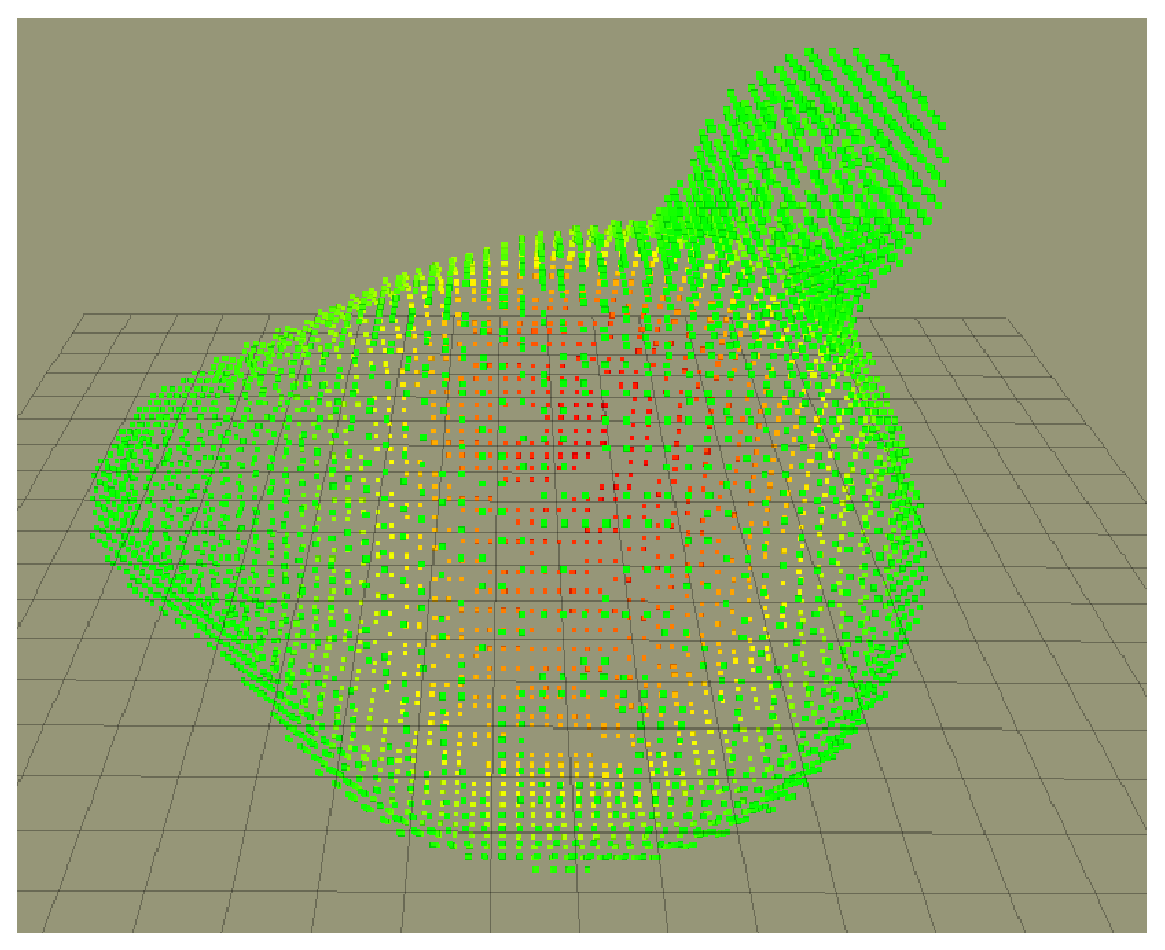
\includegraphics[width=0.9\linewidth]{example.eps}
  \caption{Different shape representations} \label{fig:shape_comparison}
\end{figure}

\begin{algorithm}[h]
\textbf{\textsc{createGaussianProcess}}($X$)\\ %functionname
\LinesNumbered
\DontPrintSemicolon
\SetAlgoVlined \SetKwInOut{Input}{input} \SetKwInOut{Output}{output}
\Input{The training data, $\mathcal{X}$, in the form of a point cloud.}
\Output{The Gaussian Process that models the object shape.}
  $\mathcal{D} \leftarrow$\textsc{deMeanNormalizeAndLabel}(\{$\mathcal{X}$, $\mathbf{0}_{\text{sizeOf}(\mathcal{X})}$\}) \\
  \textsc{addLabeledPoint}(\{$\mathbf{0}_3, -1\}$, $\mathcal{D}$) \\
  \textsc{addLabeledPoints}(\{\textsc{sphere}$(\mathbf{0}_3, 1.1, N)$, $+\mathbf{1}_{N}\}$, $\mathcal{D}$) \\
  $\mathcal{G} \leftarrow$ \textsc{doRegression}($\mathcal{D}$) \\
  \Return $\mathcal{G}$ \\
\caption{Gaussian Process regression} \label{algo:strategy}
\end{algorithm}

%%%%%%%%%%%%%%%%%%%%%%%%%%%%%%%%%%%%%%%%
\subsection{Exploration strategy}
\label{sec:strategy}

We don't need all the conditions described in \citet[Fig.~8]{Jaillet2013Path}.

\begin{algorithm}[h]
\textbf{\textsc{exploreGPAtlasRRT}}($\mathcal{M}$, $\Omega$)\\ %functionname
\LinesNumbered
\DontPrintSemicolon
\SetAlgoVlined \SetKwInOut{Input}{input} \SetKwInOut{Output}{output}
\Input{A Gaussian Process model, $\mathcal{M}$ and the set of criteria to decide how to search and end the exploration, $\Omega$.}
\Output{The best next action, $\mathcal{P}$, in the form of a path, if any, or $\varnothing$ otherwise.}
  $\mathcal{P} \leftarrow \emptyset$ \\
  $\mathcal{A} \leftarrow$\textsc{initGPAtlas}($\mathcal{M}$) \\
  $\mathcal{T} \leftarrow$\textsc{initRRTs}($\mathcal{A}$) \\
  $\mathbf{x}_{c,i} \leftarrow$\textsc{selectStartPoint}($\mathcal{M}$)\\
  $\mathcal{C}_{i} \leftarrow$\textsc{createChart}($\mathcal{A}$, $\mathbf{x}_{c,i}$, $\Omega$)\\
  \While{ \textsc{terminationCriteriaNotMet}($\mathcal{C}_{i}$, $\Omega$)}
  {
    $\mathcal{C}_{j} \leftarrow$\textsc{selectChartToExpand}($\mathcal{T}$, $\Omega$) \\
    $\mathbf{x}_{c,k} \leftarrow$\textsc{findExpansion}($\mathcal{A}$, $\mathcal{C}_{j}$, $\Omega$) \\ 
    $\mathcal{C}_{k} \leftarrow$\textsc{createChart}($\mathcal{A}$, $\mathbf{x}_{c,k}$, $\Omega$) \\ 
    \textsc{connectCharts}($\mathcal{T}$, $\mathcal{C}_{k}$, $\mathcal{C}_{j}$) \\
    $\mathcal{C}_{i} = \mathcal{C}_{k}$ \\
  }
  \eIf {\textsc{isSolution}($\mathcal{C}_{i}$)}
  {\Return $\mathcal{P} \leftarrow$\textsc{generatePath}($\mathcal{C}_{i}, \mathcal{T}$)}
  {\Return $\varnothing$}
\caption{Best-next tactile action planner} \label{alg:strategy}
\end{algorithm}

The exploration strategy, employs  the concept of RRTs and builds
an Atlas on  the Gaussian Process surface, $\mathcal{S}$. Then  it decides which
is  the  best next  tactile  action  to perform  in  order to improve the  current
object shape estimation.  Algorithm~\ref{alg:strategy}  describes  the
implemented procedure.

Specifically, given an Atlas($\mathcal{A}$), as a collection of Charts $\mathcal{C}_{i}$,
and a RRT explorer ($\mathcal{T}$) the strategy creates a starting chart on a
random point $\mathbf{x}_{c,i} \in \mathcal{M}$, belonging to the object training set($\chi$),
which in turn is part of the Gaussian Process Model ($\mathcal{M}$).
Then it rapidly builds an exploration tree on the object estimated surface until a solution
chart is found or the maximum allowed number of charts has been reached.
The solution, if found, is then the path from the chart to the tree root.

In order to do this, the atlas must be able to create new charts on the estimated surface
according to a supplied criteria ($\Omega$) and the current Gaussian Process model ($\mathcal{M}$).
Consequently a chart, must also contains a point on the surface, called the center $\mathbf{x}_c$,
such that $\mathbb{E}(\mathcal{S}(\mathbf{x}_c)) \approx 0$, a search space defined by a
tangent disc at the surface, centered on $\mathbf{x}_c$, with radius $R \propto \frac{1}{\mathbb{V}(\mathcal{S}(\mathbf{x}_c))}$ 
and finally the gradient information at the center $G \approx \frac{\partial \mathcal{S}}{\partial \mathbf{x}}$.

With such information we first ask the RRT explorer to select a chart to expand,
among the chart collection ($\mathcal{A}$).
This is done this by selecting one at random with a bias to increase the probability
of selecting the last created chart. This criteria is adopted to grow a tree
which is likely to expand on a single branch, but at the same time maintain the
possibility to create new branches from previous charts. So efficiency and speed
is preserved, while we make sure we are exploring as much surface as possible,
before reaching to a solution.

After a chart ($\mathcal{C}_j$) is selected, it is expanded by 
sampling $k$ points on its tangent discs then selecting one at maximum variance
and at the same time, not in collision with other charts search spaces. 
So a sample $\mathbf{s}_i$ is selected if $\mathbb{V}(\mathcal{S}(\mathbf{s}_i))$ is $\mathit{max}$ in $\mathbb{V}(\mathcal{S}(\mathbf{s}_k))$
and ${\parallel\mathbf{s}_i - \mathbf{x}_{c,j}\parallel}_{2} > \mathcal{C}_j \rightarrow R$, $\forall \mathcal{C}_j \in \mathcal{A}$, with $i \ne j$.

$\mathbf{s}_i$ is then projected back on the surface, using a gradient descend method,
creating a center for a new chart, $\mathbf{x}_{c,k}$.

The new chart is created and connected to the one which originated it, progressively
growing a tree of charts on the object surface.
when one reaches the termination criteria, the procedure terminates and the full
path from the converging chart to the root of the tree is reported as a solution.

The area covered by a given chart on the surface is never empty, and
it always includes the center of the chart, $\mathbf{x}_{i}$, but its shape 
depends on the local shape. However, in this work, we are not interested in computing this area, 
since we will be traversing trees using compliance control to compensate for the errors between 
linear interpolation between $\mathbf{x}_i$ and $\mathbf{x}_j$ in 3D and actual arbitrary 
shape countour joinning them.

%%%%%%%%%%%%%%%%%%%%%%%%%%%%%%%%%%%%%%%%
\subsection{Solution in a nutshell}
\label{sec:summary}

The methods from the previous sections are independent from each other, being the last one, Algorithm~\ref{alg:strategy}, our main contribution. Here, we show an example of how these methods intercommunicate to estimate the shape of an unkonwn object.

\begin{algorithm}[h]
\textbf{\textsc{ObjectShapeExploration}}$(P, \mathbb{V}_{des})$\\ %functionname
\LinesNumbered
\DontPrintSemicolon
\SetAlgoVlined \SetKwInOut{Input}{input} \SetKwInOut{Output}{output}
\Input{An initial point cloud of the scene, $P$, if any, for instance from visual object segmentation, and the desired variance, $\mathbb{V}_{des}$, for the overall shape estimation.}
\Output{The estimated object shape, $\mathcal{S}$}
  $\mathcal{S} \leftarrow \emptyset$ \\
  \If{ \textsc{isEmpty}$(P)$ }
  {
    $\chi \leftarrow $ \textsc{naiveProbe}() \\
  }
  \Else
  {
    $\chi \leftarrow $ \textsc{segmentObject}($P$) \\
  }
  $\mathcal{S} \leftarrow $\textsc{createGaussianProcess}($\chi$) \\
  \While { \texttt{true} } 
  {
    $\Gamma \leftarrow $\textsc{exploreGPAtlasRRT}$(\mathcal{S}, \mathbb{V}_{des})$ \label{exploration} \\
    \If{ $\Gamma = \emptyset$ }
    {
      \Return {$\mathcal{S}$} \label{solutionfound} \label{end} \\
    }
    \Else
    {
      \textsc{ApproachTo}($\Gamma$) \label{approach} \\
      $\bar{\chi} \leftarrow $\textsc{probeObject}($\Gamma$) \label{probe} \\
      \If{ \textsc{wasContactDetected}() }
      {
        $\upsilon \leftarrow \mathbf{0}_{\text{sizeOf}(\bar{\chi})}$  \label{belonglabel} \\
      }
      \Else
      {
        $\upsilon \leftarrow \mathbf{1}_{\text{sizeOf}(\bar{\chi})}$ \label{nobelonglabel} \\
      }
      \textsc{addLabelPoints}(\{$\bar{\chi}$, $\upsilon$\}, $\chi$) \\
      $\mathcal{S} \leftarrow $\textsc{createGaussianProcess}($\chi$) \\
      \textsc{MoveAway}() \label{away} \\
    }
  }
\caption{Probabilistic object shape modelling} \label{alg:solution}
\end{algorithm}

During the \textsc{ApproachTo} (line~\ref{approach}) (\textsc{MoveAway}, line~\ref{away}) phases, the robot uses position control and standard motion planning techniques with collision avoidance. Since we are modelling the shape, we need to ensure that everytime the robot moves close (away) from the object, it does not collide with the object. It is tentative to use the current estimated shape, but since we are not actually computing it explicitly in our approach, we choose the bounding sphere as the collision geometry of the object. Thus the robot moves towards (away from) the surface at the contact location in the normal direction until reaching the bounding sphere. After that, a standard motion planning is used to approach the object (get to the rest position).

The \textsc{probeObject} (line~\ref{probe}) phase is engaged once the robot is within the bounding sphere. The robot uses Cartesian impedance control, with the Cartesian force, pose and impedance set properly for the given setup. These implementation details are given in the next section. Since we don't actually know where the surface is, we need to whether the robot actually touched something or not, in order to properly label the acquisition (lines~\ref{belonglabel} and~\ref{nobelonglabel}) 

The method finishes when \textsc{exploreGPAtlasRRT} (line~\ref{exploration}) described in Algorithm~\ref{algo:strategy} has explore sufficiently the estimated shape and could not find an exploratory action $\Gamma$ (line~\ref{end}), i.e. the object shape is probabilistically estimated within the 95\% of the confidence interval computed from $\mathbb{V}_{des}$. 

The complete solution of the problem as stated in~\ref{sec:scope} is depicted in Algorithm~\ref{alg:solution}.

\subsection{Parameters  and probabilistic completeness}
\label{sec:analsys}

We can safely assume that the surface has only one component when seen as a manifold.
